\subsection{UNIFORMITIES ON A TOPOLOGICAL DIVISION RING}

If K is a topological division ring it is necessary to distinguish between: 1) the uniformity of the additive group of K, which is defined on K and is called the additive uniformity of K; and 2) the left and right uniformities of the multiplicative group \(\mathbf{K}^*\) , which are defined on \(\mathbf{K}^*\) and are called (by abuse of language) the multiplicative uniformities of K.

The uniformity induced on \(K^{*}\) by the additive uniformity of K is in general distinct from the multiplicative uniformities of K (see Exercise 17).

By Proposition 6, a Hausdorff topological division ring K can be considered as a dense subring of a complete Hausdorff ring \(\hat{K}\) . In order that \(\hat{K}\) should be a topological division ring it is necessary that the mapping \(x \to x^{-1}\) be extendable by continuity to \((\hat{\mathbf{K}})^{*}\) ; and this necessary condition is also sufficient, for the functions \(xx^{-1}, x^{-1}x\) and \(1\) are then equal on \((\hat{\mathbf{K}})^{*}\) by reason of the principle of extension of identities, and therefore the value of the extended function is the inverse of \(x\) for each \(x \neq 0\) in \(\hat{\mathbf{K}}\) . In other words (cf.~Chapter II, § 3, no. 6, Proposition 11):

PROPOSITION 7. The completion \(\hat{\mathbf{K}}\) of a Hausdorff topological division ring \(\mathbf{K}\) is a topological division ring if and only if the image under the mapping \(x \to x^{-1}\) of every Cauchy filter (with respect to the additive structure) which does not have a cluster point at 0, is a Cauchy filter (with respect to the additive structure).

\pandocbounded{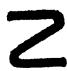
\includegraphics[keepaspectratio]{images/part002_56877e98.jpg}}

There are topological division rings in which this condition is not satisfied and in which the ring \(\hat{\mathbf{K}}\) has zero divisors (see Exercise 26). Moreover, even if the completion \(\hat{\mathbf{K}}\) is a topological division ring, there is no a priori reason to assume that the multiplicative structures of \(\hat{\mathbf{K}}\) are structures of a complete space. However, this will be the case for division rings \(\mathbf{K}\) such that \(\hat{\mathbf{K}}\) is locally compact (see Chapter I, § 9, no. 7, Proposition 13, and Chapter III, § 3, no. 3, Proposition 4) and for topological fields; for the latter, we have the following proposition:

PROPOSITION 8. If the additive uniform structure of a topological field K is a structure of a complete Hausdorff space, then the multiplicative structure on \(K^{*}\) is a structure of a complete space.

We shall show that if \(\mathfrak{F}\) is a Cauchy filter with respect to the multiplicative structure on \(\mathbf{K}^*\) , then \(\mathfrak{F}\) is a Cauchy filter with respect to the additive structure on \(\mathbf{K}\) , and does not converge to \(o\) ; this will establish the result. Let \(\mathbf{U}\) be any neighbourhood of \(o\) in \(\mathbf{K}\) , let \(\mathbf{V}\) be a closed neighbourhood of \(o\) such that \(\mathbf{V} \subset \mathbf{U}\) , \(\mathbf{VV} \subset \mathbf{U}\) {[}axiom \((\mathrm{AV}_{\mathrm{II}})]\) and \(-1 \notin V\) ; then by hypothesis there is a set \(\mathbf{A} \in \mathfrak{F}\) such that, for all \(x \in \mathbf{A}\) and \(y \in \mathbf{A}\) , we have \(x^{-1}y \in 1 + V\) . Let \(a \in \mathbf{A}\) , then \(\mathbf{A} \subset a + aV\) , and \(a + aV\) is a closed set which does not contain \(o\) ; hence \(o\) is not in the closure of \(\mathbf{A}\) and is therefore not a cluster point of \(\mathfrak{F}\) . Let \(\mathbf{W}\) be a neighbourhood of \(o\) such that \(aW \subset V\) {[}axiom \((\mathrm{AV}_{\mathrm{I}})]\) ; then by hypothesis there is a set \(\mathbf{B} \in \mathfrak{F}\) such that \(\mathbf{B} \subset \mathbf{A}\) and, for all \(x \in B\) and \(y \in B\) , we have \(x^{-1}y \in 1 + W\) ; hence \(y - x \in xW \subset AW \subset aW + aVW\) ; but \(\mathbf{K}\) is commutative, and therefore \(aVW = aWV \subset VV \subset U\) ; consequently \(y - x \in U + U\) and the Proposition is proved.

The same proof shows that Proposition 8 can be extended to the case in which every Cauchy filter with respect to one of the multiplicative structures of K is also a Cauchy filter with respect to the other multiplicative structure.

